\documentclass{article}

\usepackage{graphicx}
\usepackage{amsfonts}
\usepackage{amssymb}
\usepackage{amsmath}

\graphicspath{ {fisica-generale/assets/} }

\begin{document}

\section{Dinamica}

La dinamica è lo studio delle forze e degli effetti sul moto.
Esistono 4 tipi di forze fondamentali:

\begin{itemize}
    \item Forza elettromagnetica
    \item Forza gravitazionale
    \item Forza "nucleare debole"
    \item Forza "nucleare forte"
\end{itemize}

\noindent
La dinamica classica si basa su tre leggi fondamentali, storicamente formalizzate da Newton.

\subsection{Prima legge}

\subsubsection{Formulazione intuitiva}

Un corpo su cui la risultante delle forze è nulla mantiene inalterato il suo stato di quiete o moto.
Questa enunciazione non è precisa, perchè tratta in modo implicito il sistema di riferimento.

\subsubsection{Formulazione precisa}

Esiste un sistema di riferimento tale che un corpo materiale che sia sufficientemente lontano da tutti gli altri corpi o è in quiete o si muove di moto rettilineo uniforme.
Tale sistema di riferimento è detto inerziale.\\

\noindent
Esistono infiniti sistemi di riferimento inerziali.
Supponendo di avere un sistema di riferimento inerziale $S$.
Prendendo $S'$ che si muove rispetto ad $S$ di moto uniforme con velocità $\vec{w}$.
Anche $S'$ è un sistema di riferimento inerziale.\\

\noindent
Se su un punto $P$ nel sistema $S$ inerziale:

$$
\vec{Q}(t) = \vec{v}(t) + \vec{Q}(t_0)
$$

\noindent
È importante determinare i sistemi di riferimento inerziali perchè la descrizione delle leggi fisiche è la stessa in tutti i sistemi di riferimento.
Questo concetto è formalizzabile nel "principio di relatività Galileiano".
Sistemi di riferimento inerziali sono un'idealizzazione.
Qualsiasi sistemi di riferimento che prendiamo in pratica ha delle "deviazioni" da un sistema di riferimento inerziale ideale.
L'importante è che gli effetti dovuti all'aver scelto un sistema non inerziali siano trascurabili rispetto al moto che si vuole descrivere.

\subsection{Seconda legge}

Un punto materiale su cui agisce una forza $\vec{F}$, accelera con un'accelerazione $\vec{a}$ proporzionale a $\vec{F}$.
La costante di proporzionalità è detta massa:

$$
\vec{F} = m \vec{a}
$$

\begin{itemize}
    \item La massa si misura in $Kg$
    \item La forza si misura in Newton $N$
\end{itemize}

\noindent
$1N$ corrispende alla forza che imprime un'accelerazione di $1 m/s^2$ ad un corpo di massa $1 Kg$.\\

\noindent
L'effetto di molte forze applicate allo stesso punto è quello di un vettore forza che è la somma di tutti i vettori forza,
e lo stesso vale per l'accelerazione.

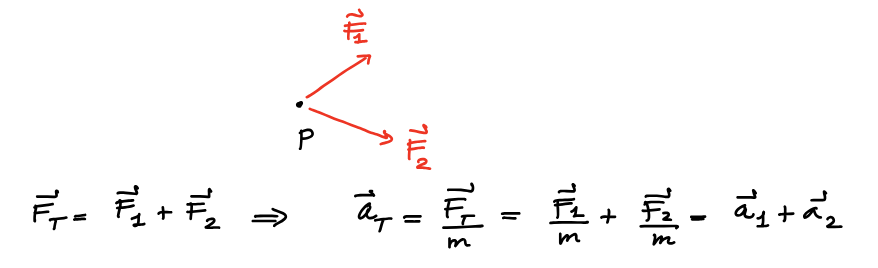
\includegraphics[width=\columnwidth]{seconda-legge-somma-forze}

\subsection{Terza legge}

Se un punto $A$ esercita una forza $\vec{F}$ su un punto $B$, allora $B$ esercita una forza $-\vec{F}$ su $A$.

\subsection{Forza elastica}

La forza elastica è quella esercitata da una molla che viene allungata o compressa rispetto a lunghezza di riposo.

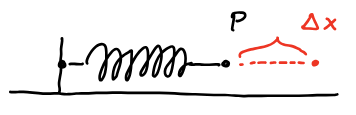
\includegraphics[width=\columnwidth]{esempio-forza-elastica}

\subsubsection{Legge di Hooke}

$$
\vec{F} = -K(\Delta x) \hat{x}
$$

\noindent
Dato $P$ di massa $m$ all'estremo della molla, ha un'accelerazione (in modulo).

$$
a = \frac{|\vec{F}|}{m} = \frac{K}{m}(\Delta x)
$$

\noindent
A differenza della forza peso, dipende da massa del corpo.

\end{document}
